\begin{figure}[ht]
    \centering
    \begin{tikzpicture}[node distance=1.5cm and 1cm, auto]
        
        % Nodo per immagine 3 con didascalia sotto, posizionato sotto img2
        \node (img3) {
            \begin{tabular}{c}
                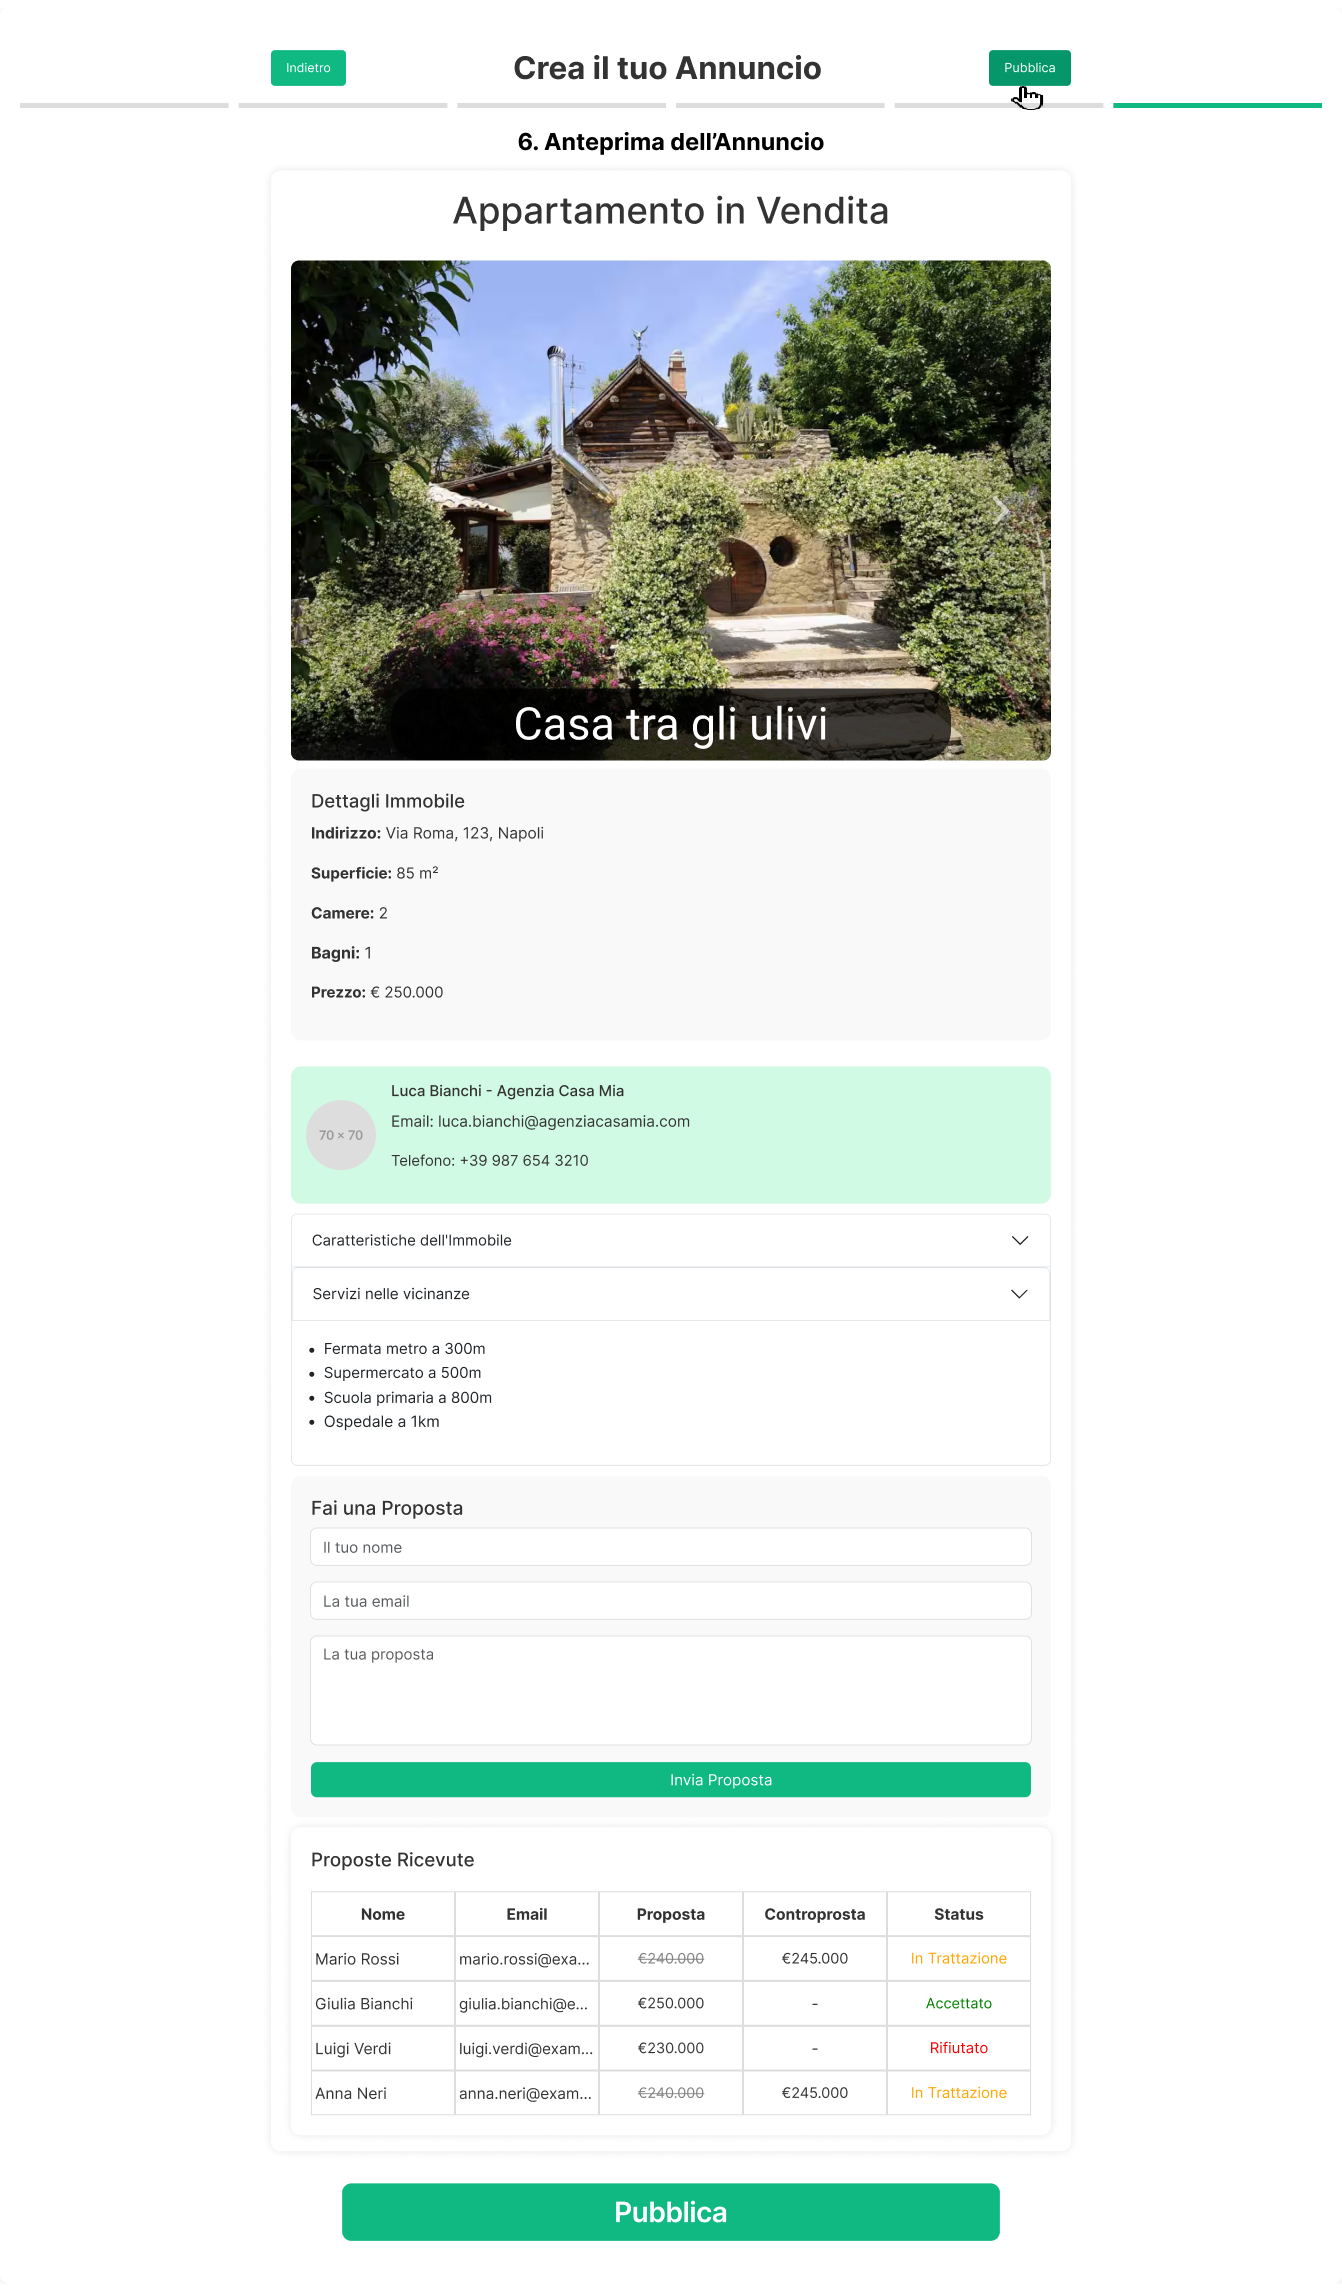
\includegraphics[width=\textwidth, height=0.8\textheight, keepaspectratio]{Immagini/Mockup/aggiungi annuncio/scenario principale/step6.png} \\
                Cockburn: step 7/8
            \end{tabular}
        };
      
    \end{tikzpicture}
    \caption{Mockup: scenario principale della tabella di Cockburn del caso d'uso nuovo annuncio.}
    \label{fig:mockup_scenario_principale_parte3_aggiungi_annuncio}
\end{figure}

\newpage

